\subsection{Réseau}

\begin{figure}[h!]
	\centering
	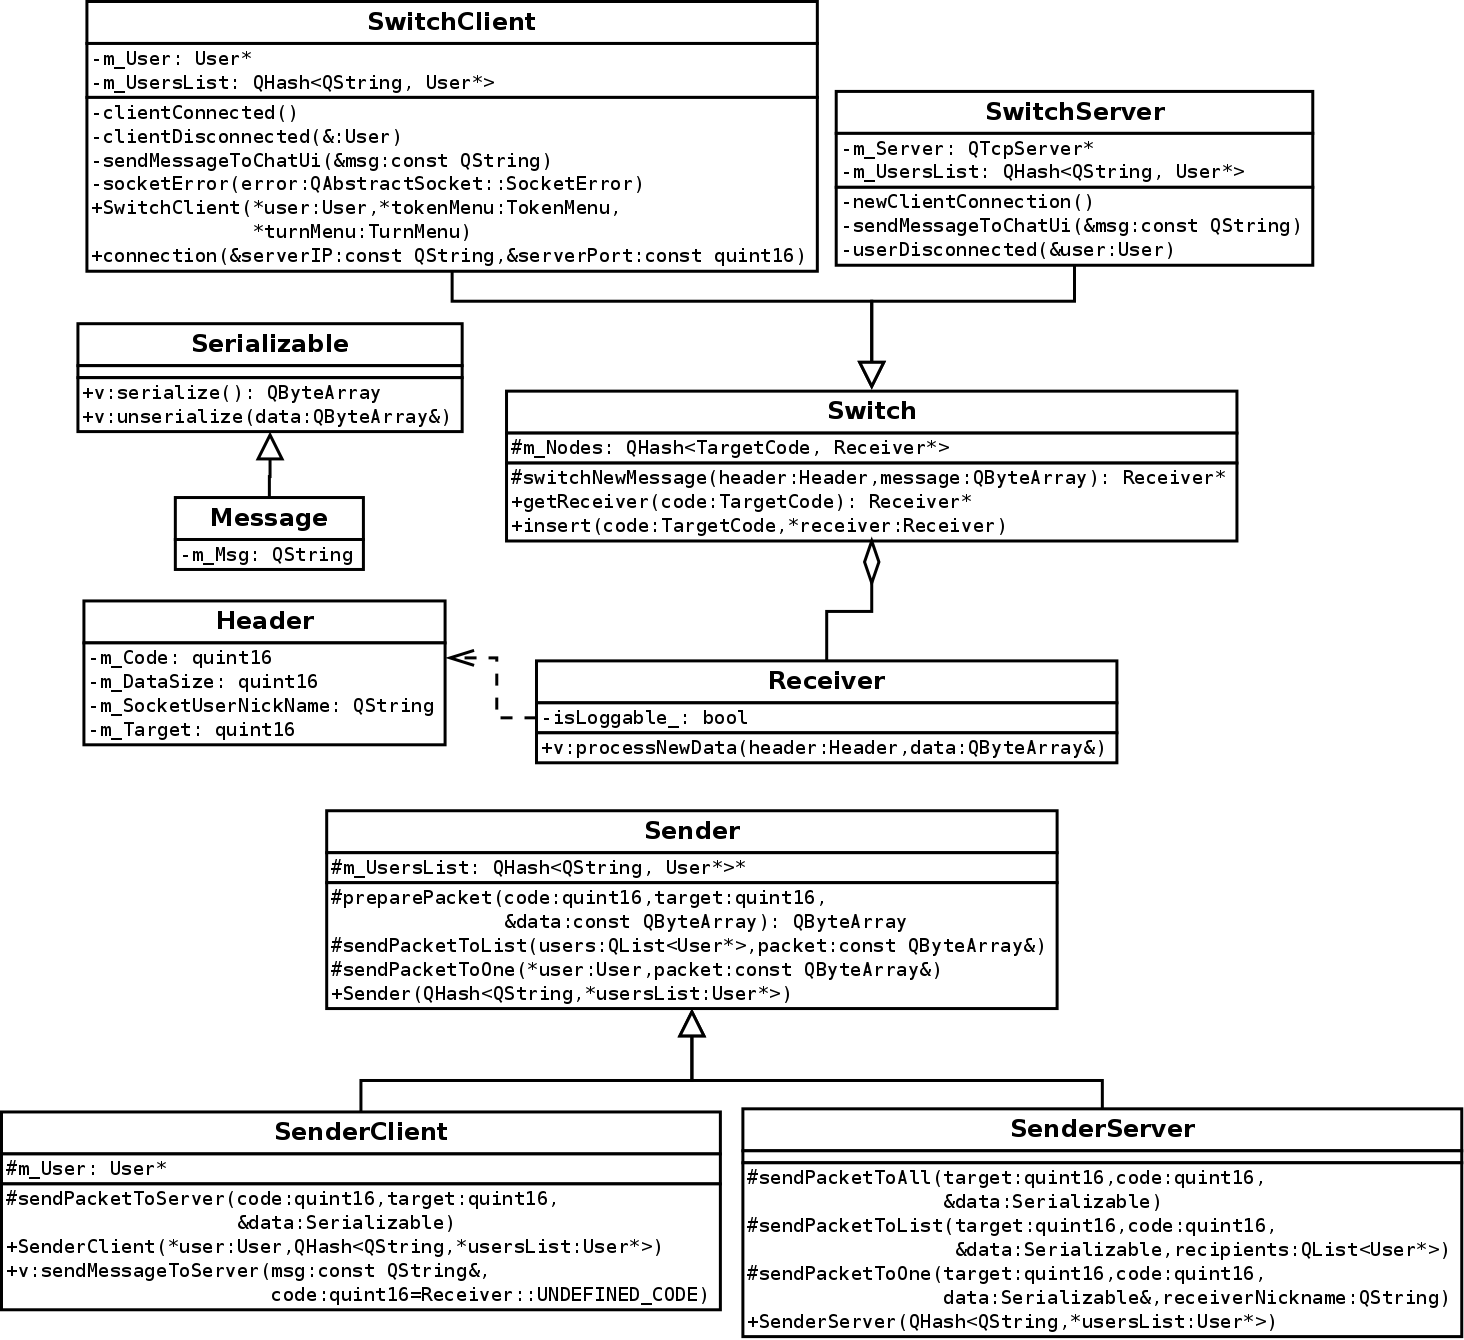
\includegraphics[width=\textwidth]{img/network_uml.png}
	\caption{Diagramme UML de la partie réseau (les modules ne sont pas représentés)}
\end{figure}

Lorsque l'application ne possédait qu'un chat, toutes les opérations nécessitant une mise en réseau se faisaient dans les classes gérant le Chat. Nous avons par la suite fait une refonte pour gérer plusieurs modules réseau en évitant de la duplication de code.\\

Nous avons tout d'abord pensé la mise en réseau sans nous occuper de la base de données. Nous avons donc cherché à pouvoir envoyer n'importe quel type d'objet. Pour cela, nous avons créé une interface Serializable possédant deux méthodes abstraites, \emph{serialize} et \emph{unserialize}. Toute classe pour laquelle nous souhaitons envoyer des objets sur le réseau doit implémenter l'interface Serializable et redéfinir les deux méthodes citées précédemment. La méthode \emph{serialize} doit stocker les attributs nécessaires à la reconstruction d'un objet de la classe dans un QByteArray. La méthode unserialize doit faire l'opération inverse, c'est à dire reconstruire un objet à partir d'un QByteArray.\\
Au final, nous n'avons que la classe Message implémentant l'interface Serializable, notre vision de la mise en réseau ayant changée pendant l'ajout de la base de donnée à l'application. En effet, notre première vision était d'envoyer des objets de classes implémentant l'interface Serializable à travers le réseau, nous aurions par exemple envoyé des objets de la classe Sprite. Cependant, avec la base de données nous avons plutôt pris l'approche suivante: les objets sont stockés en base de données, puis une notification est envoyé à toutes les applications afin que celles-ci récupèrent les nouvelles données présentes dans la base de données distante.\\

Pour communiquer, nous devons utiliser des sockets. Nous utilisons les classes présentes dans Qt: QTcpServer et QTcpSocket. Une QTcpSocket peut se connecter à un QTcpServer, et le QTcpServer reçoit un signal exploitable lorsqu'un client se connecte à lui. A travers ces sockets, des paquets sont envoyés. Nos paquet sont organisés de la manière suivante :\\

\begin{figure}[h!]
	\centering
	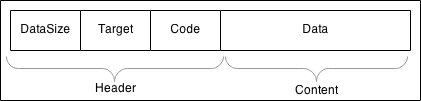
\includegraphics[scale=0.6]{img/network_packet.png}
	\caption{Structure d'un paquet}
\end{figure}

Un Header contient tout d'abord la taille de la donnée qui va être reçue, ce qui est nécessaire pour savoir lors de la réception si le paquet reçu est complet ou s'il faut attendre d'avoir reçu de nouvelles données. La Target correspond à un entier identifiant le module qui doit recevoir le paquet. Le Code correspond à l'action qui doit être effectuée par le module à qui le paquet à été transféré.\\

Lorsqu'un message est reçu, celui-ci passe par une classe héritant de Switch: SwitchClient ou SwitchServer. Ces classes sont les premières à recevoir le message et décident du module sur lequel le message doit être envoyé à l'aide de la target dans le header du paquet.\\

Les modules qui reçoivent des paquets héritent de Sender et Receiver. Un Receiver reçoit une donnée d'un Switch et la traite en exécutant des actions (méthode \emph{processNewData}). Un sender peut envoyer un paquet à une ou plusieurs sockets: un SenderClient pourra envoyer un paquet à la socket du serveur, et un SenderServer pourra envoyer un paquet à une ou plusieurs Socket(s) qui sont connectées à la socket serveur.\\

\subsubsection{MapClient \& MapServer}
Les cartes font partie des éléments mis en réseau dans l'application. La classe MapClient regarde le code du paquet reçu et exécute une action spécifique en fonction du code reçu. La classe MapServer quant à elle se contente de redistribuer les paquets qu'elle reçoit à toutes les applications (sauf l'émetteur du paquet reçu par MapServer).\\

Les actions disponibles sont les suivantes :
\begin{description}
	\item[Ouverture d'une carte] Le message reçu pour cette action contient l'id de la carte à ouvrir. Cette carte est récupérée de la base de données grâce à son id et est envoyée à la fenêtre principale pour que les initialisations nécessaires soit effectuées.
	\item[Ajout d'un sprite] L'action d'ajout d'un sprite récupère tout d'abord le sprite à ajouter de la base de données grâce à son id, récupère le jeton associé parmi les jetons déjà chargés dans l'applications et récupère la couche sur laquelle le sprite doit être posé avant de l'y ajouter.
	\item[Suppression d'un sprite] Le message de cette action contient l'id du sprite à supprimer et l'id de la couche sur laquelle celui-ci se situe. Cette couche est tout d'abord récupérée parmi les couches déjà chargées par l'application, puis nous récupérons le jeton posé sur cette couche grâce à son id. Une fois le pointeur vers ce jeton récupéré, celui-ci est supprimé.
	\item[Suppression de tous le FoW] Cette action fonctionne sur le même principe que la suppression d'un sprite, la couche de brouillard de guerre est tout d'abord récupérée grâce à son id, puis tous les sprites de cette couche sont supprimés.
	\item[Mise à jour de la couche de dessin] La couche de dessin ayant été mise à jour est tout d'abord récupérée de la base de données, puis la pixmap (image) en est extraite. Cette pixmap est remplacée dans la couche de dessin concernée.
	\item[Ping] Un message contenant l'id de la couche sur laquelle afficher le ping, ainsi que sa position en x et en y est reçu. L'action récupère ces informations, et fait appel à l'outil de ping de la couche de dessin concernée en lui passant la position en paramètre.
\end{description}
\bigskip

Ces actions sont de simples méthodes dans la classe MapClient, une évolution possible aurait été de créer une classe Action, avec plusieurs classes héritant de celle-ci pour les différentes actions de MapClient. Ces actions auraient été créées lors d'un événement sur la carte (par exemple un clic de souris pour ajouter un jeton), puis envoyées via le réseau, puis exécutées sur les différents clients lors de la réception. Cela aurait eu plusieurs bénéfices : 
\begin{itemize}
	\item ces actions auraient été génériques, afin d'être réutilisées pour tous les modules réseau de l'application;
	\item ces actions auraient pu être réversibles (une liste au niveau de MapServer garderait une trace des actions effectuées);
	\item logger les actions aurait été plus simple qu'à l'heure actuelle.
\end{itemize}
\bigskip

De plus, l'ordre dans lequel les étapes sont effectuées pour ces actions est difficilement exploitable, notamment pour des fonctionnalités de modérations. Prenons l'exemple de l'ajout d'un Sprite sur une carte décrit sur la figure \ref{fig:network_addsprite}.

\begin{figure}[h!]
	\centering
	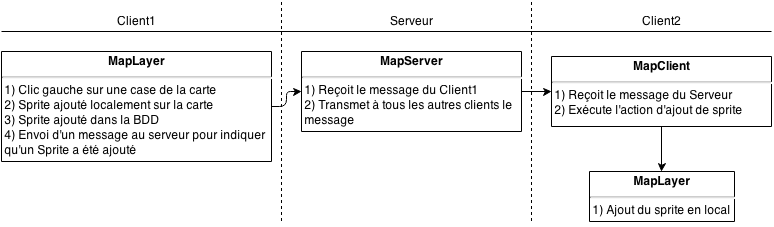
\includegraphics[width=1.0\textwidth]{img/network_addsprite.png}
	\caption{Etapes pour l'ajout d'un Sprite}
	\label{fig:network_addsprite}
\end{figure}

Dans le cas actuel décrit ci-dessus, sur un clic gauche de la souris sur la carte, un sprite est ajouté sur la carte localement et en base de données. Cependant, si nous voulons effectuer de la modération du côté du serveur, cela complique la tâche : en effet le sprite a déjà été ajouté à un client et en base de données. Il faudrait que les étapes s'effectuent comme sur le schéma ci-dessous :

\begin{figure}[h!]
	\centering
	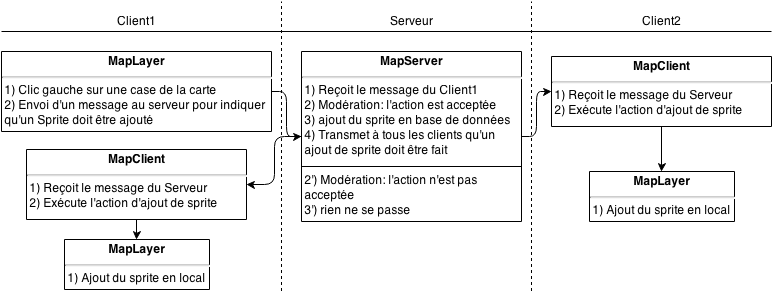
\includegraphics[width=1.0\textwidth]{img/network_addsprite_better.png}
	\caption{Etapes pour l'ajout d'un Sprite (amélioré)}
\end{figure}

\textbf{N.B.} TokenMenuClient, TokenMenuServer, TurnMenuClient et TurnMenuServer reprennent le même principe que MapClient et MapServer et ne sont donc pas détaillés.

\subsubsection{ChatClient \& ChatServer}
Les classes ChatClient et ChatServer récupèrent le code présent dans le header d'un paquet reçu et récupèrent la commande associée. Une commande est représentée par un objet d'une classe héritant de AbstractCmd. Le principe du Chat ainsi que les différentes commandes sont détaillés dans la sous-section concernant le Chat dans la section aspects techniques. Nous pouvons cependant noter que ChatClient et ChatServer utilisent des commandes, tandis que MapClient, MapServer et les autres modules utilisent des actions sous forme de méthode. Comme détaillé précédémment, il aurait été judicieux de créer des classes héritant d'une classe de base Action qui soit générique afin d'être réutilisable dans toute l'application, contrairement aux commandes qui sont fortement liées au chat.